\chapter{Verificaci\'{o}n y evaluaci\'{o}n}
En este cap\'itulo se detallar\'an las pruebas
que se han llevado a cabo para verificar que el software
cumple todos los requisitos correctamente.

Las pruebas representan los comportamientos que debe
tener la aplicaci\'on, es decir, lo que se prueban son los
casos de uso y subcasos de uso, no si cada m\'etodo
realiza de forma correcta su tarea.

\section{Cargar XML}

\subsection{Preparaci\'on de las pruebas}
Para poder probar este comportamiento no se requiere de ninguna preparaci\'on 
especial.

\subsection{Cargar XML v\'alido nada m\'as abrir la aplicaci\'on}
Se prueba el comportamiento que debe tener la aplicaci\'on al cargar
un XML para empezar a trabajar, lo que se conoce como un arranque en fr\'io.

\paragraph{Resultado esperado}
Todos los datos cargados en la aplicaci\'on eliminados, 
tanto intervalos creados, como visualizadores de datos,
contenedores... todo debe haberse borrado de memoria volviendo a un estado inicial
de la aplicaci\'on.

\paragraph{Resultado obtenido}
Todos los datos se han borrado excepto los elementos del \'arbol de observaciones
y propiedades. 

\paragraph{Acciones realizadas}
Modificado el m\'etodo de cargar XML para limpiar tambi\'en los elementos del
\'arbol.

\subsection{Cargar XML v\'alido cuando ya haya un XML cargado}
Esta prueba contempla dos situaciones, 
ya que este comportamiento se da cuando hay
hay un XML cargado pero no se ha hecho nada, como cuando hay un XML cargado justo
despu\'es de guardar un paso o situaci\'on a disco.

\paragraph{Resultado esperado}
Todos los datos cargados en la aplicaci\'on eliminados, 
tanto intervalos creados, como visualizadores de datos,
contenedores... todo debe haberse borrado de memoria volviendo a un estado inicial
de la aplicaci\'on.

\paragraph{Resultado obtenido}
Todos los datos se han borrado.

\paragraph{Acciones realizadas}
Ninguna.

\subsection{Cargar XML v\'alido habiendo un XML cargado y con uno o varios intervalos guardados}
Esta prueba contempla el hecho de cargar un XML cuando ya hemos creado uno o varios
intervalos listos para ser guardados

\paragraph{Resultado esperado}
Todos los datos cargados en la aplicaci\'on eliminados, sobre todo dando mucha importancia a
que se eliminen los intervalos.

\paragraph{Resultado obtenido}
Todos los datos se han eliminado correctamente.

\paragraph{Acciones realizadas}
Ninguna por obtener el resultado esperado.

\subsection{Cargar un XML no v\'alido}
Se utiliza para comprobar si la funci\'on de validaci\'on funciona correctamente.

\paragraph{Resultado esperado}
Se mostrar\'a un error informando de que el XML que se ha intentado cargar
no valida contra el XSD.

\paragraph{Resultado obtenido}
El archivo se valida e intenta cargarse produciendo una
excepci\'on.

\paragraph{Acciones realizadas}
Se revisa tanto el c\'odigo de validaci\'on como el XSD para descubrir
d\'onde estaba el fallo. Finalmente se descubri\'o que el fallo estaba en el
XSD por lo que se arregla para que valide correctamente.

\section{Crear intervalo}
\subsection{Preparaci\'on de las pruebas}
Para poder crear un intervalo es necesario tener cargado un XML, y adem\'as haber cargado,
al menos, una propiedad en el sistema y tener un rango seleccionado.

\subsection{Guardar el rango no habiendo ninguno guardado previamente}
Se probar\'a si guarda correctamente un rango cu\'ando no hay ninguno guardado de antes.
Aqu\'i se pone a prueba el comportamiento de cuando se van a guardar rangos que no entran
en conflicto con ninguno.

\paragraph{Resultado esperado}
El rango se guarda en la colecci\'on de intervalos a guardar en disco, y se 
muestra un mensaje informando de que se ha a\~nadido correctamente.

\paragraph{Resultado obtenido}
El resultado obtenido es el esperado, se ha a\~nadido correctamente y se muestra
el mensaje de informaci\'on

\paragraph{Acciones realizadas}
Ninguna al obtener el resultado esperado

\subsection{Guardar un rango que solape a otro previamente guardado}
Esta prueba contiene a su vez cuatro pruebas que han sido agrupadas, ya que un intervalo
se puede superponer a otro de cuatro maneras, tal y como se ve en la Figura \ref{fig:ModosSolapamiento}.

\begin{figure}[H]
\centering
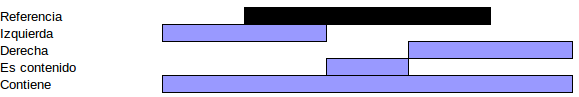
\includegraphics[width=0.9\linewidth]{./Figures/ModosSolapamiento.png}
\caption{Modos solapamiento}
\label{fig:ModosSolapamiento}
\end{figure}

El cuadrado negro representa el intervalo que est\'a guardado en el sistema, y 
los azules-lilas representan el que va a intentarse guardar.

\paragraph{Resultado esperado}
Las cuatro veces que intenten guardarse esos intervalos debe salir un mensaje informando
de que el intervalo a guardar solapa con alguno previamente guardado, y no debe
guardarse.

\paragraph{Resultado obtenido}
Para esos cuatro casos se obtiene el resultado esperado, pero en el caso extremo
en el que el intervalo guardado y el intervalo a guardar son iguales se guarda, dando
lugar a incongruencias. Hay que tener en cuenta que en el caso de empezar y acabar
en el mismo punto es la situaci\'on de ``contiene".

\paragraph{Acciones realizadas}
Se ajustan las comprobaciones, se cambian los ``<" \ y ``>" \ por ``$\leq$" \ y ``$\geq$".

\subsection{Guardar un intervalo vac\'io}
Lo que se prueba aqu\'i es que no se pueda guardar un intervalo vac\'io, ya que ser\'ia
llenar el XML resultante con etiquetas vac\'ias. Para probar se seleccionar\'a un rango
vac\'io y se pinchar\'a en crear intervalo.

\paragraph{Resultado esperado}
Un mensaje de advertencia indicando que es necesario seleccionar un rango, y
el intervalo no se guardar\'a.

\paragraph{Resultado obtenido}
No se muestra nada y se guarda el intervalo

\paragraph{Acciones realizadas}
Se crea la condici\'on en la que se muestre el
di\'alogo y que no se guarde nada, si el inicio del intervalo
es igual al final del intervalo.

\section{Guardar paso o situaci\'on}
\subsection{Preparaci\'on de las pruebas}
Para guardar un paso o situaci\'on, no se necesita ninguna preparaci\'on especial.
Para guardar un paso o una situaci\'on que tenga sentido, se requiere 
haber creado al menos un 
intervalo. 

\subsection{Guardar paso o situaci\'on}
Al pinchar en guardar paso, se mostrar\'a el di\'alogo de guardado.
Dependiendo de si el usuario quiere guardar o no, se realizar\'a una
acci\'on u otra.

\paragraph{Resultado esperado}
Si el usuario decide guardar, se guardar\'an todos los intervalos
creados previamente y se descargar\'an de memoria. Si no se decide
guardar, no se har\'a nada y se podr\'a seguir trabajando.

\paragraph{Resultado obtenido}
Los resultados son los esperados.

\paragraph{Acciones realizadas}
Ninguna.

\section{A\~nadir v\'ideo}
\subsection{Preparaci\'on de las pruebas}
Para a\~nadir un v\'ideo no se requiere de acciones previas.
Se pueden a\~nadir en cualquier momento.

\subsection{A\~nadir un v\'ideo que no existe}
Al a\~nadir un v\'ideo que no existe, se a\~nade a la lista
de v\'ideos cargados.

\paragraph{Resultado esperado}
El v\'ideo se a\~nade.

\paragraph{Resultado obtenido}
El v\'ideo es a\~nadido

\paragraph{Acciones realizadas}
Ninguna.

\subsection{A\~nadir un v\'ideo que ya existe}
Al a\~nadir un v\'ideo que ya existe, no se a\~nade
a la lista de v\'ideos cargados.

\paragraph{Resultado esperado}
El v\'ideo no se a\~nade a la vista de v\'ideos
cargados y adem\'as no se a\~nade a la lista
de v\'ideos cargados.

\paragraph{Resultado obtenido}
El v\'ideo se a\~nade tanto a la vista como a la lista
de v\'ideos cargados.

\paragraph{Acciones realizadas}
Implementadas las interfaces \texttt{IEquatable<T>} e \texttt{IComparable<T>}
utilizando como m\'etodo de comparaci\'on el nombre del archivo cargado.
Se requieren esas dos interfaces para que el \'arbol rojo-negro funcione correctamente.
En el caso de \texttt{IComparable<T>} se ordena alfab\'eticamente por nombre
del archivo cargado.

\section{Cargar propiedad u observaci\'on}
Todas las pruebas tienen en com\'un que al ser cargadas deben mostrar
el rango seleccionado por otras propiedades ya en memoria.
\subsection{Preparaci\'on de las pruebas}
Para poder cargar una propiedad u observaci\'on es requisito
indispensable que haya sido cargado un XML v\'alido

\subsection{Cargar una propiedad no cargada}
Al cargar una propiedad no cargada previamente
se prueba el comportamiento por defecto de la aplicaci\'on.

\paragraph{Resultado esperado}
La propiedad se a\~nade junto a su observaci\'on
si no estaba a\~nadida. Si no, simplemente se a\~nade la propiedad
a la observaci\'on que corresponde. Adem\'as en memoria tambi\'en
se habr\'an cargado correctamente.

\paragraph{Resultado obtenido}
El resultado es el esperado.

\paragraph{Acciones realizadas}
Ninguna.

\subsection{Cargar una propiedad ya cargada}
En esta situaci\'on se prueba cuando la propiedad
ya est\'a cargada y el usuario intenta volver a cargarla

\paragraph{Resultado esperado}
La propiedad no debe cargarse ni visualmente ni en memoria.

\paragraph{Resultado obtenido}
la propiedad no se carga visualmente pero si en memoria, y el software
al no ser consciente de que ese dato ha sido cargado, causa una fuga de memoria
pudiendo dejar al pc sin memoria disponible.

\paragraph{Acciones realizadas}
Se sigue paso a paso la ejecuci\'on hasta descubrir que la comprobaci\'on
de si ya estaba cargada se realizaba contra el objeto equivocado, causando que
siempre pod\'ia ser a\~nadido. Se sustituy\'o por un \'arbol rojo-negro
porque una de sus propiedades es que s\'olo puede haber un objeto de cada.
Tambi\'en se implementaron las mismas interfaces que a los v\'ideos, utilizando
como comparaci\'on el nombre de la propiedad, al igual que para insertarlo
en el \'arbol.

\subsection{Cargar una observaci\'on no cargada}
Igual que con la propiedad, solo que al cargar una observaci\'on
se a\~naden tanto la observaci\'on como todas las propiedades. Tambi\'en
se puede realizar esta acci\'on cuando algunas propiedades de la observaci\'on
ya han sido cargadas.

\paragraph{Resultado esperado}
Si nada de esa observaci\'on hab\'ia sido cargado previamente, se a\~nadir\'an
todas las propiedades de esa observaci\'on tanto en memoria como visualmente.

Si ya hab\'ia alguna propiedad de esa observaci\'on cargada, se a\~nadir\'an las
restantes.

\paragraph{Resultado obtenido}
El resultado es el esperado.

\paragraph{Acciones realizadas}
Ninguna.

\subsection{Cargar una observaci\'on ya cargada}
Podr\'ia considerarse un subcaso de la prueba anterior. Pero se va a 
considerar que una observaci\'on cargada es aquella que tiene todas sus 
propiedades a\~nadidas al sistema.

\paragraph{Resultado esperado}
No debe suceder nada, las propiedades al ya estar cargadas no deben a\~nadirse
ni en memoria ni visualmente.

\paragraph{Resultado obtenido}
El esperado.

\paragraph{Acciones realizadas}
Ninguna.

\section{Cerrar observaci\'on}
\subsection{Preparaci\'on de las pruebas}
Para poder cerrar una observaci\'on, se requiere cargar un XML v\'alido y
adem\'as haber a\~nadido por lo menos una propiedad.

\subsection{Cerrar observaci\'on}
Al pinchar sobre la ``X" \ de la esquina superior derecha de la observaci\'on,
se quitar\'a de vista y de memoria.

\paragraph{Resultados esperados}
La observaci\'on se quita de la vista y todas las propiedades asociadas se eliminar\'an
de memoria y de la vista tambi\'en.

\paragraph{Resultados obtenidos}
Se borran de la vista pero no se borran de memoria causando otra fuga de memoria.

\paragraph{Acciones realizadas}
Revisar donde puede fallar y a\~nadir un evento que cuando se este ocultando en la
vista, elimine la observaci\'on, y con ello, todas las propiedades de memoria.

\section{Cerrar propiedad}
\subsection{Preparaci\'on de las pruebas}
Para poder cerrar una observaci\'on, se requiere cargar un XML v\'alido y
adem\'as haber a\~nadido por lo menos una propiedad.

\subsection{Cerrar propiedad}
Al pinchar sobre la ``X" \ de la esquina superior derecha de la propiedad,
se quitar\'a de vista y de memoria.

\paragraph{Resultados esperados}
La propiedad se quita de la vista y de memoria.

\paragraph{Resultados obtenidos}
El resultado es el esperado.

\paragraph{Acciones realizadas}
Ninguna.

\section{Seleccionar rango}
\subsection{Preparaci\'on de las pruebas}
Se requiere cargar de al menos cuatro propiedades para probar el funcionamiento
completo. Dos de una observaci\'on, y dos de otra.

\subsection{Seleccionar un rango}
En cualquiera de las propiedades abiertas pinchar y arrastrar para seleccionar
un rango.

\paragraph{Resultados esperados}
El resto de propiedades deben sincronizar con el rango autom\'aticamente.

\paragraph{Resultados obtenidos}
En l\'ogica el valor ha cambiado pero el gr\'afico no se refresca.

\paragraph{Acciones realizadas}
Investigar la manera de refrescar manualmente los gr\'aficos.
Finalmente se descubre que la funci\'on \texttt{InvalidatePlot(true)} realiza
esa tarea.